\PassOptionsToPackage{unicode=true}{hyperref} % options for packages loaded elsewhere
\PassOptionsToPackage{hyphens}{url}
%
\documentclass[]{article}
\usepackage{lmodern}
\usepackage{amssymb,amsmath}
\usepackage{ifxetex,ifluatex}
\usepackage{fixltx2e} % provides \textsubscript
\ifnum 0\ifxetex 1\fi\ifluatex 1\fi=0 % if pdftex
  \usepackage[T1]{fontenc}
  \usepackage[utf8]{inputenc}
  \usepackage{textcomp} % provides euro and other symbols
\else % if luatex or xelatex
  \usepackage{unicode-math}
  \defaultfontfeatures{Ligatures=TeX,Scale=MatchLowercase}
\fi
% use upquote if available, for straight quotes in verbatim environments
\IfFileExists{upquote.sty}{\usepackage{upquote}}{}
% use microtype if available
\IfFileExists{microtype.sty}{%
\usepackage[]{microtype}
\UseMicrotypeSet[protrusion]{basicmath} % disable protrusion for tt fonts
}{}
\IfFileExists{parskip.sty}{%
\usepackage{parskip}
}{% else
\setlength{\parindent}{0pt}
\setlength{\parskip}{6pt plus 2pt minus 1pt}
}
\usepackage{hyperref}
\hypersetup{
            pdftitle={Model Questions},
            pdfauthor={Thiyanga Talagala},
            pdfborder={0 0 0},
            breaklinks=true}
\urlstyle{same}  % don't use monospace font for urls
\usepackage[margin=1in]{geometry}
\usepackage{color}
\usepackage{fancyvrb}
\newcommand{\VerbBar}{|}
\newcommand{\VERB}{\Verb[commandchars=\\\{\}]}
\DefineVerbatimEnvironment{Highlighting}{Verbatim}{commandchars=\\\{\}}
% Add ',fontsize=\small' for more characters per line
\usepackage{framed}
\definecolor{shadecolor}{RGB}{248,248,248}
\newenvironment{Shaded}{\begin{snugshade}}{\end{snugshade}}
\newcommand{\AlertTok}[1]{\textcolor[rgb]{0.94,0.16,0.16}{#1}}
\newcommand{\AnnotationTok}[1]{\textcolor[rgb]{0.56,0.35,0.01}{\textbf{\textit{#1}}}}
\newcommand{\AttributeTok}[1]{\textcolor[rgb]{0.77,0.63,0.00}{#1}}
\newcommand{\BaseNTok}[1]{\textcolor[rgb]{0.00,0.00,0.81}{#1}}
\newcommand{\BuiltInTok}[1]{#1}
\newcommand{\CharTok}[1]{\textcolor[rgb]{0.31,0.60,0.02}{#1}}
\newcommand{\CommentTok}[1]{\textcolor[rgb]{0.56,0.35,0.01}{\textit{#1}}}
\newcommand{\CommentVarTok}[1]{\textcolor[rgb]{0.56,0.35,0.01}{\textbf{\textit{#1}}}}
\newcommand{\ConstantTok}[1]{\textcolor[rgb]{0.00,0.00,0.00}{#1}}
\newcommand{\ControlFlowTok}[1]{\textcolor[rgb]{0.13,0.29,0.53}{\textbf{#1}}}
\newcommand{\DataTypeTok}[1]{\textcolor[rgb]{0.13,0.29,0.53}{#1}}
\newcommand{\DecValTok}[1]{\textcolor[rgb]{0.00,0.00,0.81}{#1}}
\newcommand{\DocumentationTok}[1]{\textcolor[rgb]{0.56,0.35,0.01}{\textbf{\textit{#1}}}}
\newcommand{\ErrorTok}[1]{\textcolor[rgb]{0.64,0.00,0.00}{\textbf{#1}}}
\newcommand{\ExtensionTok}[1]{#1}
\newcommand{\FloatTok}[1]{\textcolor[rgb]{0.00,0.00,0.81}{#1}}
\newcommand{\FunctionTok}[1]{\textcolor[rgb]{0.00,0.00,0.00}{#1}}
\newcommand{\ImportTok}[1]{#1}
\newcommand{\InformationTok}[1]{\textcolor[rgb]{0.56,0.35,0.01}{\textbf{\textit{#1}}}}
\newcommand{\KeywordTok}[1]{\textcolor[rgb]{0.13,0.29,0.53}{\textbf{#1}}}
\newcommand{\NormalTok}[1]{#1}
\newcommand{\OperatorTok}[1]{\textcolor[rgb]{0.81,0.36,0.00}{\textbf{#1}}}
\newcommand{\OtherTok}[1]{\textcolor[rgb]{0.56,0.35,0.01}{#1}}
\newcommand{\PreprocessorTok}[1]{\textcolor[rgb]{0.56,0.35,0.01}{\textit{#1}}}
\newcommand{\RegionMarkerTok}[1]{#1}
\newcommand{\SpecialCharTok}[1]{\textcolor[rgb]{0.00,0.00,0.00}{#1}}
\newcommand{\SpecialStringTok}[1]{\textcolor[rgb]{0.31,0.60,0.02}{#1}}
\newcommand{\StringTok}[1]{\textcolor[rgb]{0.31,0.60,0.02}{#1}}
\newcommand{\VariableTok}[1]{\textcolor[rgb]{0.00,0.00,0.00}{#1}}
\newcommand{\VerbatimStringTok}[1]{\textcolor[rgb]{0.31,0.60,0.02}{#1}}
\newcommand{\WarningTok}[1]{\textcolor[rgb]{0.56,0.35,0.01}{\textbf{\textit{#1}}}}
\usepackage{graphicx,grffile}
\makeatletter
\def\maxwidth{\ifdim\Gin@nat@width>\linewidth\linewidth\else\Gin@nat@width\fi}
\def\maxheight{\ifdim\Gin@nat@height>\textheight\textheight\else\Gin@nat@height\fi}
\makeatother
% Scale images if necessary, so that they will not overflow the page
% margins by default, and it is still possible to overwrite the defaults
% using explicit options in \includegraphics[width, height, ...]{}
\setkeys{Gin}{width=\maxwidth,height=\maxheight,keepaspectratio}
\setlength{\emergencystretch}{3em}  % prevent overfull lines
\providecommand{\tightlist}{%
  \setlength{\itemsep}{0pt}\setlength{\parskip}{0pt}}
\setcounter{secnumdepth}{0}
% Redefines (sub)paragraphs to behave more like sections
\ifx\paragraph\undefined\else
\let\oldparagraph\paragraph
\renewcommand{\paragraph}[1]{\oldparagraph{#1}\mbox{}}
\fi
\ifx\subparagraph\undefined\else
\let\oldsubparagraph\subparagraph
\renewcommand{\subparagraph}[1]{\oldsubparagraph{#1}\mbox{}}
\fi

% set default figure placement to htbp
\makeatletter
\def\fps@figure{htbp}
\makeatother

\usepackage{etoolbox}
\makeatletter
\providecommand{\subtitle}[1]{% add subtitle to \maketitle
  \apptocmd{\@title}{\par {\large #1 \par}}{}{}
}
\makeatother

\title{Model Questions}
\providecommand{\subtitle}[1]{}
\subtitle{STA 506 2.0 Linear Regression Analysis}
\author{Thiyanga Talagala}
\date{05/12/2020}

\begin{document}
\maketitle

Answers: in class discussion on 12 Dec 2020.

\hypertarget{use-5-significance-level-for-all-tests.}{%
\subsection{Use 5\% significance level for all
tests.}\label{use-5-significance-level-for-all-tests.}}

\hypertarget{question-1}{%
\subsection{Question 1}\label{question-1}}

A chemical reaction is performed at different levels of temperature
(Celsius) and the end product is weighed (g). The following results were
obtained for the purpose of finding a regression model to represent the
relationship of the two variables.

\begin{verbatim}
   Temperature Weight
1           10     11
2           10      9
3           20     16
4           33     23
5           33     24
6           40     25
7           40     26
8           40     23
9           47     25
10          50     22
11          56     26
12          56     27
13          56     26
14          60     25
15          60     27
16          65     24
17          69     24
\end{verbatim}

\begin{enumerate}
\def\labelenumi{\roman{enumi})}
\tightlist
\item
  The two variables are supposed to have a linear relationship. Write
  the model you would fit to these data.
\end{enumerate}

\newpage

\textcolor{blue}{Answer}

\newpage

A regression analysis was performed with these data and the following
outputs were obtained using R.

\textbf{Output a}

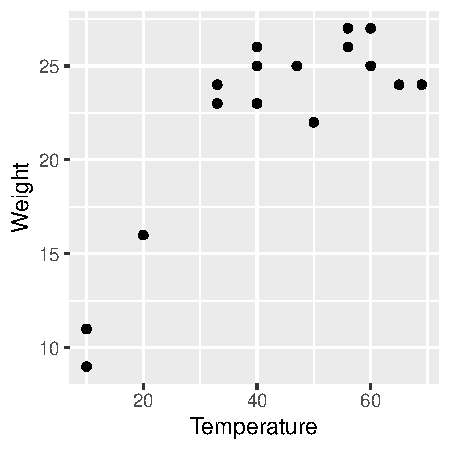
\includegraphics{modelquestions_discussions_files/figure-latex/unnamed-chunk-2-1.pdf}

\textbf{Output b}

\begin{verbatim}

Call:
lm(formula = Weight ~ Temperature, data = df)

Residuals:
    Min      1Q  Median      3Q     Max 
-5.2450 -2.0422  0.4882  1.6926  4.4071 

Coefficients:
            Estimate Std. Error t value Pr(>|t|)    
(Intercept) 11.79572    2.03828   5.787 3.58e-05 ***
Temperature  0.24493    0.04318   5.672 4.43e-05 ***
---
Signif. codes:  0 '***' 0.001 '**' 0.01 '*' 0.05 '.' 0.1 ' ' 1

Residual standard error: 3.123 on 15 degrees of freedom
Multiple R-squared:  0.682, Adjusted R-squared:  0.6608 
F-statistic: 32.18 on 1 and 15 DF,  p-value: 4.429e-05
\end{verbatim}

\textbf{Output c}

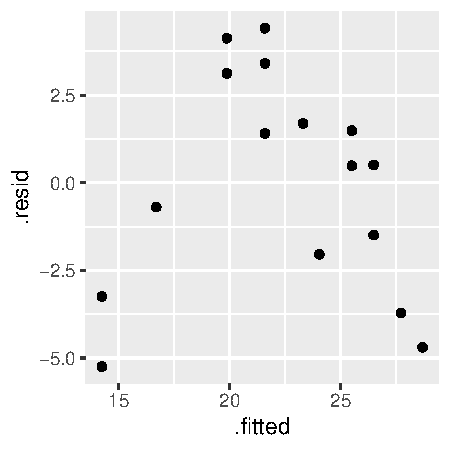
\includegraphics{modelquestions_discussions_files/figure-latex/unnamed-chunk-4-1.pdf}

\textbf{Output d}

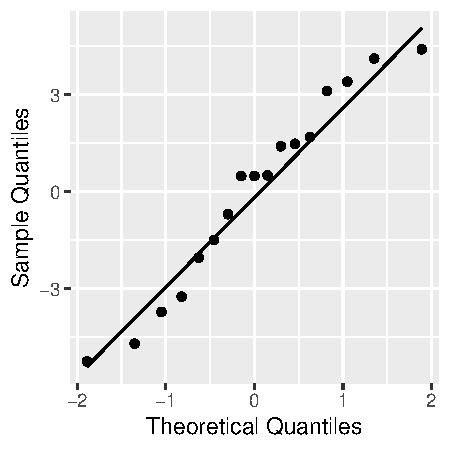
\includegraphics{modelquestions_discussions_files/figure-latex/unnamed-chunk-5-1.pdf}

\textbf{Output e}

\begin{verbatim}

    Shapiro-Wilk normality test

data:  fitmodel$.resid
W = 0.95278, p-value = 0.502
\end{verbatim}

\begin{enumerate}
\def\labelenumi{\roman{enumi})}
\setcounter{enumi}{1}
\tightlist
\item
  Two undergraduates studying statistics were looking at this analysis.
\end{enumerate}

\begin{enumerate}
\def\labelenumi{(\Alph{enumi})}
\item
  One said that the results strongly suggest that this model is highly
  significant and can be used for prediction purposes.
\item
  The other said that the results show the fitted model is not
  appropriate for this case and this model cannot be used for
  prediction.
\end{enumerate}

With whom would you agree? Justify your argument using each part ((a) to
(e)) of the results given.

\textcolor{blue}{Answer}

\newpage

\hypertarget{question-2}{%
\subsection{Question 2}\label{question-2}}

In a soap production factory, there are two machines used for the
production. Using 27 production runs; 15 of line 1 and 12 of line 2, the
management wanted to find the relationship between the machine speed and
the amount of scrap produced during the production process. To allow the
two machines have different regression lines with different intercepts
and slopes the following model was fitted with all 27 observations.

\[Y = \beta_0 + \beta_1 X_1 + \beta_2 X_2 + \beta_3 X_1 X_2 + \epsilon\]

where,

\(X_1\) is line speed and

\begin{equation}
  X_{2} =
  \begin{cases}
    1 & \text{if line 1} \\
    0 & \text{if line 2}
  \end{cases}
\end{equation}

\begin{enumerate}
\def\labelenumi{\roman{enumi})}
\tightlist
\item
  Draw a sketch of the scatter plot which is expected with the above
  model.
\end{enumerate}

\textcolor{blue}{Answer}

\newpage

\textcolor{blue}{Answer}

\newpage

\begin{enumerate}
\def\labelenumi{\roman{enumi})}
\setcounter{enumi}{1}
\tightlist
\item
  Write the model for each line.
\end{enumerate}

\textcolor{blue}{Answer}

\newpage

\begin{enumerate}
\def\labelenumi{\roman{enumi})}
\setcounter{enumi}{2}
\tightlist
\item
  Write the hypotheses that should be tested to find whether the two
  machines have the same regression model or not, i.e.~whether both the
  intercept and the slope are the same of the two models you wrote in
  ii) in the above.
\end{enumerate}

\textcolor{blue}{Answer}

\newpage

\hypertarget{question-3}{%
\subsection{Question 3}\label{question-3}}

A group of new graduates who have studied Statistics, Mathematics and
Computer Science at the Faculty of Applied Sciences of University of
Jayewardenepura joined a company. They were given three tests in the
three subjects they have studied for the degree at the final interview
at which they were selected for the job. After three months of a
probationary period, their proficiency for the job was measured. The
tests scores and the measure of proficiency were analysed to find a
model to predict proficiency by the test scores. Some results are shown
below.

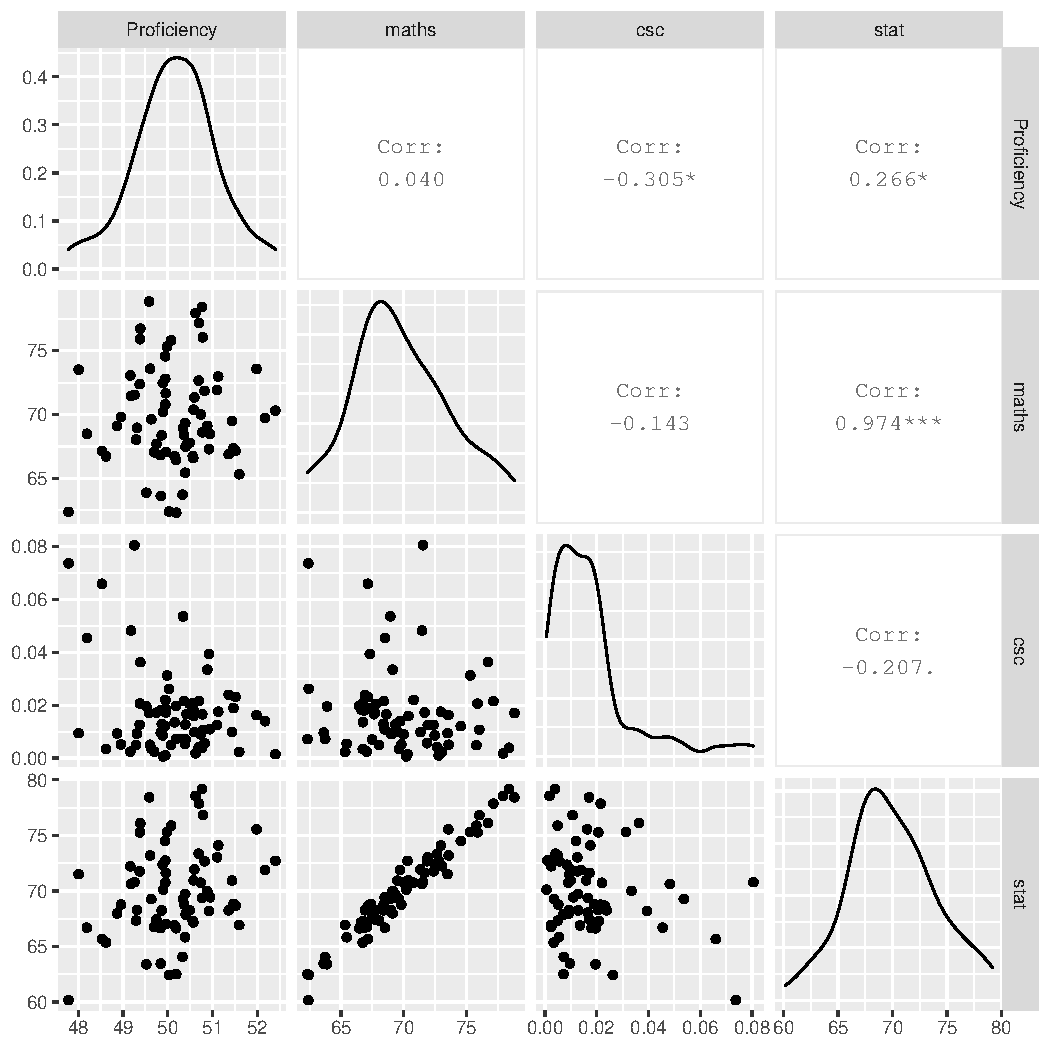
\includegraphics{modelquestions_discussions_files/figure-latex/unnamed-chunk-7-1.pdf}

\begin{Shaded}
\begin{Highlighting}[]
\NormalTok{model.sjp <-}\StringTok{ }\KeywordTok{lm}\NormalTok{(Proficiency }\OperatorTok{~}\StringTok{ }\NormalTok{maths }\OperatorTok{+}\StringTok{ }\NormalTok{csc }\OperatorTok{+}\StringTok{ }\NormalTok{stat, }\DataTypeTok{data=}\NormalTok{df)}
\KeywordTok{summary}\NormalTok{(model.sjp)}
\end{Highlighting}
\end{Shaded}

\begin{verbatim}

Call:
lm(formula = Proficiency ~ maths + csc + stat, data = df)

Residuals:
       Min         1Q     Median         3Q        Max 
-1.136e-13  5.390e-16  2.112e-15  2.632e-15  9.808e-15 

Coefficients:
              Estimate Std. Error    t value Pr(>|t|)    
(Intercept)  5.000e+01  3.311e-14  1.510e+15   <2e-16 ***
maths       -1.000e+00  2.113e-15 -4.732e+14   <2e-16 ***
csc          1.647e-14  1.175e-13  1.400e-01    0.889    
stat         1.000e+00  2.062e-15  4.849e+14   <2e-16 ***
---
Signif. codes:  0 '***' 0.001 '**' 0.01 '*' 0.05 '.' 0.1 ' ' 1

Residual standard error: 1.51e-14 on 66 degrees of freedom
Multiple R-squared:      1, Adjusted R-squared:      1 
F-statistic: 8.644e+28 on 3 and 66 DF,  p-value: < 2.2e-16
\end{verbatim}

\begin{Shaded}
\begin{Highlighting}[]
\NormalTok{car}\OperatorTok{::}\KeywordTok{vif}\NormalTok{(model.sjp)}
\end{Highlighting}
\end{Shaded}

\begin{verbatim}
    maths       csc      stat 
20.786453  1.123955 21.276288 
\end{verbatim}

A statistician examined these results and claimed that
``multicollinearity'' has affected this model.

\begin{enumerate}
\def\labelenumi{\roman{enumi})}
\tightlist
\item
  What is meant by multicollinearity?
\end{enumerate}

\textcolor{blue}{Answer}

\newpage

\textcolor{blue}{Answer}

\newpage

\begin{enumerate}
\def\labelenumi{\roman{enumi})}
\setcounter{enumi}{1}
\tightlist
\item
  Do you agree with statistician claim. Justify your answer.
\end{enumerate}

\textcolor{blue}{Answer}

\newpage

The following outputs are obtained using R

\begin{Shaded}
\begin{Highlighting}[]
\KeywordTok{as.data.frame}\NormalTok{(}\KeywordTok{augment}\NormalTok{(model.sjp))}
\end{Highlighting}
\end{Shaded}

\begin{verbatim}
   Proficiency    maths          csc     stat  .fitted       .resid  .std.resid
1     49.37355 72.37755 0.0125863639 71.75109 49.37355 2.842171e-14 -7.66025591
2     50.18364 66.45027 0.0196940463 66.63391 50.18364 2.131628e-14 -1.48070338
3     49.16437 73.05363 0.0024284454 72.21800 49.16437 2.842171e-14  0.10714738
4     51.59528 65.32951 0.0023299210 66.92479 51.59528 2.842171e-14  0.51401085
5     50.32951 63.73183 0.0072678104 64.06134 50.32951 2.842171e-14  0.15099172
6     49.17953 71.45723 0.0482494756 70.63676 49.17953 2.842171e-14  0.11353877
7     50.48743 67.78354 0.0204927009 68.27097 50.48743 3.552714e-14  0.61154678
8     50.73832 70.00553 0.0089947140 70.74385 50.73832 2.842171e-14  0.15314500
9     50.57578 70.37171 0.0159427916 70.94749 50.57578 2.842171e-14  0.15526421
10    49.69461 67.05240 0.0024507665 66.74701 49.69461 2.842171e-14  0.11058196
11    51.51178 67.15666 0.0231789188 68.66844 51.51178 2.131628e-14 -0.30393684
12    50.38984 69.32411 0.0127004976 69.71395 50.38984 2.131628e-14 -0.32222317
13    49.37876 75.89043 0.0206267258 75.26919 49.37876 3.552714e-14  0.64620513
14    47.78530 62.38217 0.0737322370 60.16747 47.78530 2.842171e-14  0.03042069
15    51.12493 72.96973 0.0175757195 74.09466 51.12493 2.842171e-14  0.20391182
16    49.95507 71.66475 0.0172540658 71.61982 49.95507 2.842171e-14  0.14220069
17    49.98381 75.31550 0.0312672529 75.29931 49.98381 2.842171e-14  0.16850045
18    50.94384 68.47908 0.0109124440 69.42292 50.94384 2.131628e-14 -0.32417535
19    50.82122 71.85009 0.0056155579 72.67132 50.82122 2.842171e-14  0.14888595
20    50.59390 71.33549 0.0098079954 71.92940 50.59390 2.131628e-14 -0.30560012
21    50.91898 67.28740 0.0394085876 68.20638 50.91898 2.842171e-14  0.14208232
22    50.78214 76.03934 0.0106982098 76.82148 50.78214 2.842171e-14  0.15521017
23    50.07456 75.80201 0.0049020065 75.87658 50.07456 2.842171e-14  0.16958165
24    48.01065 73.50107 0.0094310921 71.51172 48.01065 3.552714e-14  0.63426528
25    50.61983 77.93417 0.0017678771 78.55399 50.61983 2.842171e-14  0.18326864
26    49.94387 72.79243 0.0009906527 72.73630 49.94387 2.842171e-14  0.16885449
27    49.84420 63.61704 0.0096452077 63.46124 49.84420 2.842171e-14  0.14829990
28    48.52925 67.13367 0.0659822142 65.66292 48.52925 3.552714e-14  0.59640621
29    49.52185 63.87694 0.0195552018 63.39879 49.52185 2.842171e-14  0.06564973
30    50.41794 67.63300 0.0166135493 68.05094 50.41794 2.131628e-14 -0.33509719
31    51.35868 66.89817 0.0239214224 68.25685 51.35868 2.131628e-14 -0.33351870
32    49.89721 70.21058 0.0006211421 70.10779 49.89721 3.552714e-14  0.61497247
33    50.38767 65.44539 0.0054001692 65.83306 50.38767 2.842171e-14  0.14562036
34    49.94619 70.79014 0.0220077988 70.73634 49.94619 2.131628e-14 -0.33447465
35    48.62294 66.72708 0.0033918392 65.35002 48.62294 3.552714e-14  0.58014681
36    49.58501 78.83644 0.0170454313 78.42144 49.58501 3.552714e-14  0.60631430
37    49.60571 73.58354 0.0050290156 73.18925 49.60571 3.552714e-14  0.59720009
38    49.94069 74.55087 0.0120869051 74.49156 49.94069 3.552714e-14  0.66207624
39    51.10003 71.92093 0.0125257115 73.02095 51.10003 2.131628e-14 -0.30981731
40    50.76318 78.41088 0.0039171242 79.17406 50.76318 2.842171e-14  0.29221843
41    49.83548 66.82132 0.0179980190 66.65679 49.83548 2.842171e-14  0.11001700
42    49.74664 67.69178 0.0171374484 67.43841 49.74664 2.842171e-14  0.13194807
43    50.69696 77.16141 0.0215376941 77.85837 50.69696 2.842171e-14  0.15740006
44    50.55666 66.74652 0.0208850892 67.30318 50.55666 2.131628e-14 -0.31794536
45    49.31124 68.96310 0.0092440233 68.27434 49.31124 2.131628e-14 -0.36156458
46    49.29250 68.03596 0.0050213833 67.32847 49.29250 3.552714e-14  0.61126880
47    50.36458 68.40004 0.0215520776 68.76462 50.36458 3.552714e-14  0.61536115
48    50.76853 68.60443 0.0165759298 69.37297 50.76853 2.842171e-14  0.14046909
49    49.88765 72.47094 0.0085695716 72.35860 49.88765 2.842171e-14  0.17312488
50    50.88111 69.11335 0.0334638734 69.99446 50.88111 2.842171e-14  0.15883595
51    50.39811 67.47021 0.0070373741 67.86832 50.39811 2.842171e-14  0.13148371
52    49.38797 76.71519 0.0363128761 76.10317 49.38797 2.842171e-14  0.16691255
53    50.34112 68.92710 0.0536298170 69.26822 50.34112 2.842171e-14  0.14600906
54    48.87064 69.10222 0.0092971559 67.97285 48.87064 2.842171e-14  0.09976906
55    51.43302 69.49905 0.0099102942 70.93207 51.43302 3.552714e-14  0.65346379
56    51.98040 73.56333 0.0162899301 75.54373 51.98040 2.131628e-14 -0.25992139
57    49.63278 69.63218 0.0034977763 69.26496 49.63278 2.842171e-14  0.12710776
58    48.95587 69.81183 0.0051574643 68.76769 48.95587 2.842171e-14  0.12718476
59    50.56972 66.59170 0.0184322711 67.16142 50.56972 2.842171e-14  0.15493337
60    49.86495 68.37865 0.0129031294 68.24359 49.86495 2.131628e-14 -0.35285094
61    52.40162 70.30080 0.0014945680 72.70242 52.40162 2.842171e-14  0.24036644
62    49.96076 67.05553 0.0184696109 67.01629 49.96076 2.842171e-14  0.10948345
63    50.68974 72.65748 0.0041210709 73.34722 50.68974 2.842171e-14  0.15930696
64    50.02800 62.40803 0.0261997808 62.43603 50.02800 2.842171e-14  0.13035356
65    49.25673 71.53279 0.0805468791 70.78952 49.25673 2.131628e-14 -0.39077805
66    50.18879 62.31775 0.0071855355 62.50654 50.18879 2.842171e-14  0.08025915
67    48.19504 68.49512 0.0455064886 66.69016 48.19504 3.552714e-14  0.61023202
68    51.46555 67.35860 0.0189471903 68.82416 51.46555 2.131628e-14 -0.33286468
69    50.15325 66.73953 0.0135561374 66.89278 50.15325 2.842171e-14  0.12200098
70    52.17261 69.71552 0.0139501082 71.88813 52.17261 2.131628e-14 -0.29376393
         .hat       .sigma      .cooksd
1  0.03491457 5.066616e-15 5.307226e-01
2  0.02523086 1.495837e-14 1.418752e-02
3  0.06256608 1.521186e-14 1.915585e-04
4  0.07669201 1.518271e-14 5.486408e-03
5  0.06006372 1.521056e-14 3.642169e-04
6  0.07585078 1.521170e-14 2.645126e-04
7  0.02118640 1.517002e-14 2.023748e-03
8  0.02170681 1.521048e-14 1.300986e-04
9  0.01751163 1.521041e-14 1.074192e-04
10 0.04671670 1.521178e-14 1.498162e-04
11 0.06134208 1.520254e-14 1.509239e-03
12 0.01638207 1.520122e-14 4.323106e-04
13 0.06085543 1.516498e-14 6.764687e-03
14 0.25137809 1.521308e-14 7.768606e-05
15 0.04135050 1.520839e-14 4.483794e-04
16 0.01821781 1.521086e-14 9.380469e-05
17 0.05858375 1.520991e-14 4.417104e-04
18 0.02748128 1.520107e-14 7.424018e-04
19 0.02828862 1.521063e-14 1.613325e-04
20 0.02064506 1.520242e-14 4.921791e-04
21 0.06759207 1.521086e-14 3.658557e-04
22 0.05587418 1.521041e-14 3.564197e-04
23 0.05378780 1.520987e-14 4.086890e-04
24 0.12589022 1.516675e-14 1.448465e-02
25 0.08316856 1.520932e-14 7.617036e-04
26 0.03894284 1.520990e-14 2.888309e-04
27 0.06199928 1.521065e-14 3.634170e-04
28 0.15392031 1.517214e-14 1.617741e-02
29 0.05478978 1.521269e-14 6.245641e-05
30 0.02027931 1.520024e-14 5.810753e-04
31 0.05575867 1.520036e-14 1.642139e-03
32 0.03525760 1.516954e-14 3.455356e-03
33 0.04441475 1.521074e-14 2.464007e-04
34 0.01688088 1.520029e-14 4.802367e-04
35 0.09649255 1.517435e-14 8.986237e-03
36 0.09788394 1.517076e-14 9.972055e-03
37 0.04402388 1.517203e-14 4.106020e-03
38 0.03723970 1.516258e-14 4.238810e-03
39 0.03288907 1.520212e-14 8.160685e-04
40 0.09001817 1.520334e-14 2.111800e-03
41 0.02484526 1.521179e-14 7.709561e-05
42 0.02205663 1.521118e-14 9.816836e-05
43 0.07572514 1.521033e-14 5.074447e-04
44 0.02736433 1.520153e-14 7.110164e-04
45 0.03744683 1.519811e-14 1.271458e-03
46 0.04921764 1.517006e-14 4.835531e-03
47 0.01826358 1.516948e-14 1.761129e-03
48 0.02250110 1.521091e-14 1.135505e-04
49 0.02702832 1.520973e-14 2.081507e-04
50 0.04677216 1.521028e-14 3.094770e-04
51 0.02738920 1.521119e-14 1.217094e-04
52 0.09128065 1.520998e-14 6.996276e-04
53 0.09704183 1.521073e-14 5.727841e-04
54 0.05691727 1.521204e-14 1.501848e-04
55 0.04220150 1.516389e-14 4.703669e-03
56 0.08826138 1.520540e-14 1.635025e-03
57 0.03618049 1.521133e-14 1.516222e-04
58 0.05991494 1.521132e-14 2.577378e-04
59 0.02772283 1.521042e-14 1.711108e-04
60 0.02052014 1.519883e-14 6.520898e-04
61 0.10042059 1.520653e-14 1.612393e-03
62 0.02226123 1.521181e-14 6.822809e-05
63 0.03095501 1.521026e-14 2.026733e-04
64 0.06744995 1.521123e-14 3.072524e-04
65 0.24356832 1.519558e-14 1.229282e-02
66 0.08013045 1.521245e-14 1.402815e-04
67 0.09760958 1.517021e-14 1.006996e-02
68 0.05324077 1.520041e-14 1.557687e-03
69 0.02530942 1.521147e-14 9.662335e-05
70 0.08633564 1.520324e-14 2.038639e-03
\end{verbatim}

\begin{enumerate}
\def\labelenumi{\roman{enumi})}
\setcounter{enumi}{2}
\tightlist
\item
  Are there any observations that have high leverage values? If so, what
  are the observation numbers.
\end{enumerate}

\textcolor{blue}{Answer}

\newpage

\textcolor{blue}{Answer}

\newpage

\begin{enumerate}
\def\labelenumi{\roman{enumi})}
\setcounter{enumi}{3}
\tightlist
\item
  Are there any observations that are outliers? If so, what are the
  sample observation numbers?
\end{enumerate}

\textcolor{blue}{Answer}

\newpage

\textcolor{blue}{Answer}

\newpage

\hypertarget{question-4}{%
\subsection{Question 4}\label{question-4}}

it is required to study the relationship between age (\(X\)) and girth
(\(Y\)) of teak trees growing in a plantation. Note that girth is the
diameter of the tree (in inches) measured at 5 inches above the ground.
The girth of the trees and the ages (in years) have been recorded from a
sample of 25 trees. Assume that the scatterplot of the data clearly
shows a linear relationship between the two variables with an intercept.

\begin{enumerate}
\def\labelenumi{\roman{enumi})}
\tightlist
\item
  Write the simple linear regression model that you would be fitted for
  the above variables. Define all terms in it and state any assumptions
  regarding the model.
\end{enumerate}

\textcolor{blue}{Answer}

\newpage

\begin{enumerate}
\def\labelenumi{\roman{enumi})}
\setcounter{enumi}{1}
\tightlist
\item
  Later it was suggested that a linear model goes through the origin is
  suitable for this situation. Write the new model using the usual
  notation.
\end{enumerate}

\textcolor{blue}{Answer}

\newpage

\begin{enumerate}
\def\labelenumi{\roman{enumi})}
\setcounter{enumi}{2}
\tightlist
\item
  The estimated regression model in part (ii) satisfied all of the
  assumptions regarding the error term. Sketch the residual plot vs
  fitted values and Q-Q normality plot of residuals.
\end{enumerate}

\textcolor{blue}{Answer}

\newpage

\hypertarget{question-5}{%
\subsection{Question 5}\label{question-5}}

An experiment was conducted to determine the influence of sulphide
concentration (\(X_1\)) on the whiteness of rayon (\(Y\)). The results
obtained through R are given below.

\begin{Shaded}
\begin{Highlighting}[]
\NormalTok{x1 <-}\StringTok{ }\KeywordTok{rnorm}\NormalTok{(}\DecValTok{15}\NormalTok{, }\DataTypeTok{mean=}\DecValTok{40}\NormalTok{)}
\NormalTok{y <-}\StringTok{ }\DecValTok{13} \OperatorTok{+}\StringTok{ }\NormalTok{(}\DecValTok{2}\OperatorTok{*}\NormalTok{x1) }\OperatorTok{+}\StringTok{ }\KeywordTok{rnorm}\NormalTok{(}\DecValTok{15}\NormalTok{)}
\NormalTok{df5 <-}\StringTok{ }\KeywordTok{data.frame}\NormalTok{(}\DataTypeTok{x1=}\NormalTok{x1, }\DataTypeTok{Y=}\NormalTok{y)}
\NormalTok{mod5 <-}\StringTok{ }\KeywordTok{lm}\NormalTok{(Y }\OperatorTok{~}\StringTok{ }\NormalTok{x1, }\DataTypeTok{data=}\NormalTok{df5)}
\KeywordTok{summary}\NormalTok{(mod5)}
\end{Highlighting}
\end{Shaded}

\begin{verbatim}

Call:
lm(formula = Y ~ x1, data = df5)

Residuals:
     Min       1Q   Median       3Q      Max 
-1.69929 -0.48179  0.02163  0.66530  1.31226 

Coefficients:
            Estimate Std. Error t value Pr(>|t|)    
(Intercept)   21.718     12.780   1.699    0.113    
x1             1.786      0.321   5.563 9.19e-05 ***
---
Signif. codes:  0 '***' 0.001 '**' 0.01 '*' 0.05 '.' 0.1 ' ' 1

Residual standard error: 0.9087 on 13 degrees of freedom
Multiple R-squared:  0.7042,    Adjusted R-squared:  0.6814 
F-statistic: 30.94 on 1 and 13 DF,  p-value: 9.185e-05
\end{verbatim}

\begin{Shaded}
\begin{Highlighting}[]
\KeywordTok{anova}\NormalTok{(mod5)}
\end{Highlighting}
\end{Shaded}

\begin{verbatim}
Analysis of Variance Table

Response: Y
          Df Sum Sq Mean Sq F value    Pr(>F)    
x1         1 25.550 25.5497  30.944 9.185e-05 ***
Residuals 13 10.734  0.8257                      
---
Signif. codes:  0 '***' 0.001 '**' 0.01 '*' 0.05 '.' 0.1 ' ' 1
\end{verbatim}

\begin{enumerate}
\def\labelenumi{\roman{enumi})}
\tightlist
\item
  Construct the ANOVA table using the above results.
\end{enumerate}

\textcolor{blue}{Answer}

\newpage

\textcolor{blue}{Answer}

\newpage

\begin{enumerate}
\def\labelenumi{\roman{enumi})}
\setcounter{enumi}{1}
\tightlist
\item
  Write the hypothesis to be tested in the ANOVA in part i.
\end{enumerate}

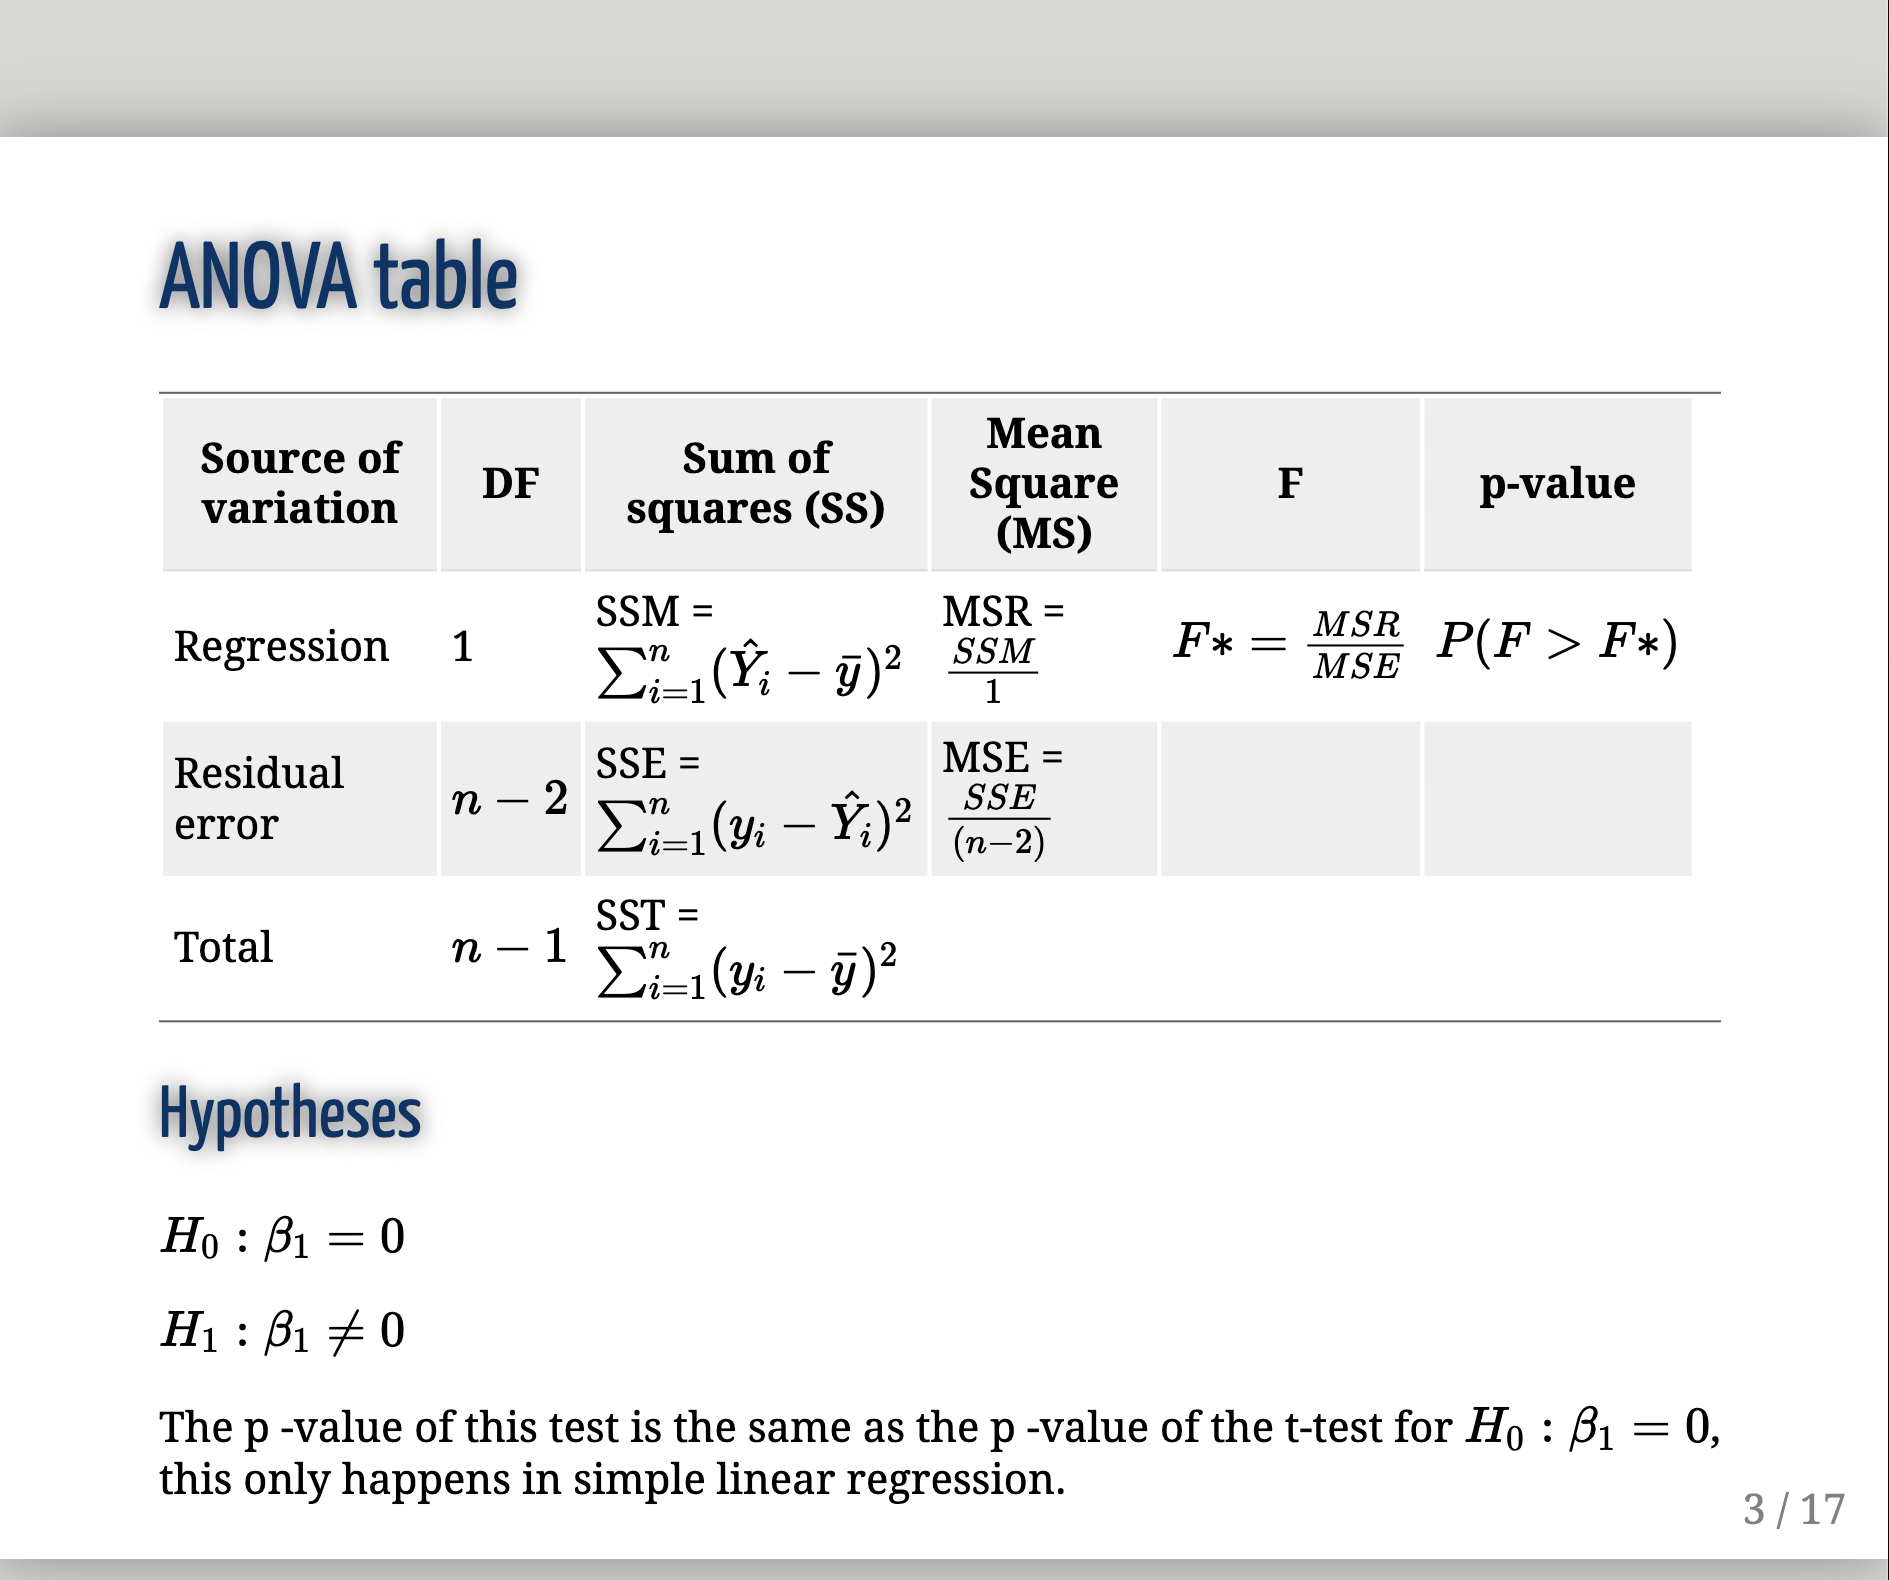
\includegraphics{ANOVA.png}

\textcolor{blue}{Answer}

\newpage

\textcolor{blue}{Answer}

\begin{enumerate}
\def\labelenumi{\roman{enumi})}
\setcounter{enumi}{2}
\tightlist
\item
  What is your decision about the fitted model.
\end{enumerate}

\newpage

\textcolor{blue}{Answer}

\end{document}
